\section{Esercizio 19}

\textit{\textbf{Descrizione:}  Calcolare (numericamente) la \emph{costante di Lebesgue} per i polinomi interpolanti di grado
$n = 2,4,6,...,40$, sia sulle ascisse equidistanti che su quelle di \emph{Chebyshev} (utilizzare 10001 punti equispaziati per valutare la funzione di Lebesgue).
Graficare convenientemente i risultati ottenuti.
Spiegare, quindi, i risultati ottenuti approssimando la funzione\\
\[
f(x)=\frac{1}{1+x^2},\ \  x \in [-5,5]
\]
utilizzando le ascisse equidistanti e di \emph{Chebyshev} precedentemente menzionate (tabulare il massimo errore valutato su una gliglia 10001 punti equidistanti nell'intervallo $[-5,5]$).}
\newline
\noindent\emph{Soluzione: }\newline
Ricordiamo che la \emph{costante di Lebesgue} $\Lambda_n$ è definita come:\\
\[
\begin{aligned}
\Lambda_n &= || \lambda_n||\\
\lambda_n(x) &= \sum_{i=0}^{n} |L_{i,n}(x)|\\
L_{i,n}(x) &= \prod_{j=0, j\neq i}^{n} \frac{x-x_j}{x_i-x_j}
\end{aligned}
\]
con $\lambda_n(x)$  \emph{funzione di Lebesgue}, $L_{i,n}(x)$ il \emph{polinomio di base di Lagrange} per l'interpolazione polinomiale e $x_0,...,x_n$ le \emph{ascisse di interpolazione}.\\
\section*{Calcolo della costante di Lebesgue}
Per il calcolo della \emph{Costante di Lebesgue}, abbiamo utilizzato il seguente \emph{Script matlab}: 
\lstinputlisting{resources/19CalcoloLebesgue.m}
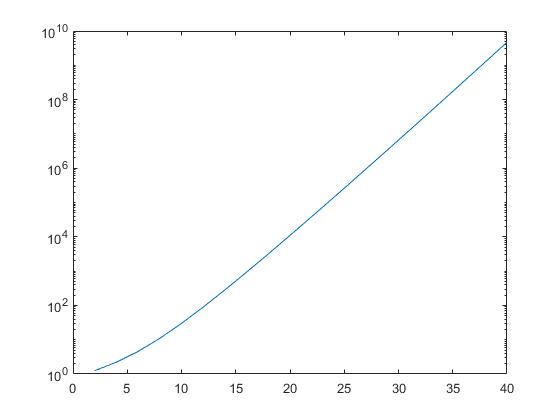
\includegraphics[width=1\linewidth]{img/19equidistanti.jpg}
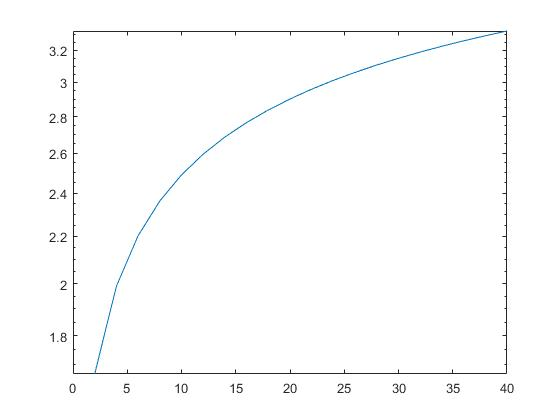
\includegraphics[width=1\linewidth]{img/19cheb.jpg}
\newpage
Per la tabulazione, è stato utilizzato il seguente \emph{script}:\\
\lstinputlisting{resources/19tabulazione.m}
Di seguito riportiamo i risultati ottenuti dall'esecuzione:\\ \\
\begin{tabular}{|c|c|c|}	% TABULAZIONE ERRORE PER ASCISSE EQUID E CHEBYSHEV
\hline
n&Ascisse Equidistanti&Ascisse di Chebyshev\\\hline
2 &$6.462292487 \cdot 10^{-1}$&$6.005977 \cdot 10^{-1}$\\ \hline
4 &$4.383571219 \cdot 10^{-1}$&$4.020169 \cdot 10^{-1}$\\ \hline
6 &$6.169479237 \cdot 10^{-1}$&$2.642274 \cdot 10^{-1}$\\ \hline
8 &$1.045176501 \cdot 10^{0}$ &$1.708356 \cdot 10^{-1}$\\ \hline
10&$1.915658802 \cdot 10^{0}$ &$1.091534 \cdot 10^{-1}$\\ \hline
12&$3.663392805 \cdot 10^{0}$ &$6.921570 \cdot 10^{-2}$\\ \hline
14&$7.194881107 \cdot 10^{0}$ &$4.660234 \cdot 10^{-2}$\\ \hline
16&$1.439385128 \cdot 10^{1}$ &$3.261358 \cdot 10^{-2}$\\ \hline
18&$2.919043772 \cdot 10^{1}$ &$2.249228 \cdot 10^{-2}$\\ \hline
20&$5.982230871 \cdot 10^{1}$ &$1.533371 \cdot 10^{-2}$\\ \hline
22&$1.236242551 \cdot 10^{2}$ &$1.035891 \cdot 10^{-2}$\\ \hline
24&$2.572129123 \cdot 10^{2}$ &$6.948423 \cdot 10^{-3}$\\ \hline
26&$5.381745497 \cdot 10^{2}$ &$4.634870 \cdot 10^{-3}$\\ \hline
28&$1.131420473 \cdot 10^{3}$ &$3.078216 \cdot 10^{-3}$\\ \hline
30&$2.388280971 \cdot 10^{3}$ &$2.061587 \cdot 10^{-3}$\\ \hline
32&$5.058959842 \cdot 10^{3}$ &$1.401747 \cdot 10^{-3}$\\ \hline
34&$1.074904570 \cdot 10^{4}$ &$9.493348 \cdot 10^{-4}$\\ \hline
36&$2.290122855 \cdot 10^{4}$ &$6.407501 \cdot 10^{-4}$\\ \hline
38&$4.890718552 \cdot 10^{4}$ &$4.312103 \cdot 10^{-4}$\\ \hline
40&$1.046676871 \cdot 10^{5}$ &$2.894608 \cdot 10^{-4}$\\ \hline
\end{tabular}
\\ \\Osservando la tabella, si nota come rispetto alle ascisse \emph{Equidistanti}, quelle di \emph{Chebyshev} vadano a minimizzare il valore di  $\Lambda_n$ al crescere di n.